\documentclass[border=6pt]{standalone}
\usepackage{amsmath,amssymb}
\usepackage{xcolor}
\usepackage{tikz}
\usetikzlibrary{arrows.meta,backgrounds}
\definecolor{cblue}{HTML}{1976D2}
\definecolor{cred}{HTML}{E53935}
\definecolor{cpurple}{HTML}{5E35B1}
\definecolor{cgrey}{HTML}{757575}
\tikzset{every picture/.append style={show background rectangle,
    background rectangle/.style={fill=white}, inner frame sep=4pt}}
% The rows of one window, drawn with W = 2: the start down the page, the lag across. Three rows are
% stored, the older ones are discarded and keep only their candidates. A candidate is an entry of the
% middle row below the threshold and below its eight neighbours. A candidate within W of a smaller one
% is dropped. A candidate within W + 1 rows of the middle row is undecided, since the middle row may
% still bring a smaller one within W, and one further back is decided.
\begin{document}
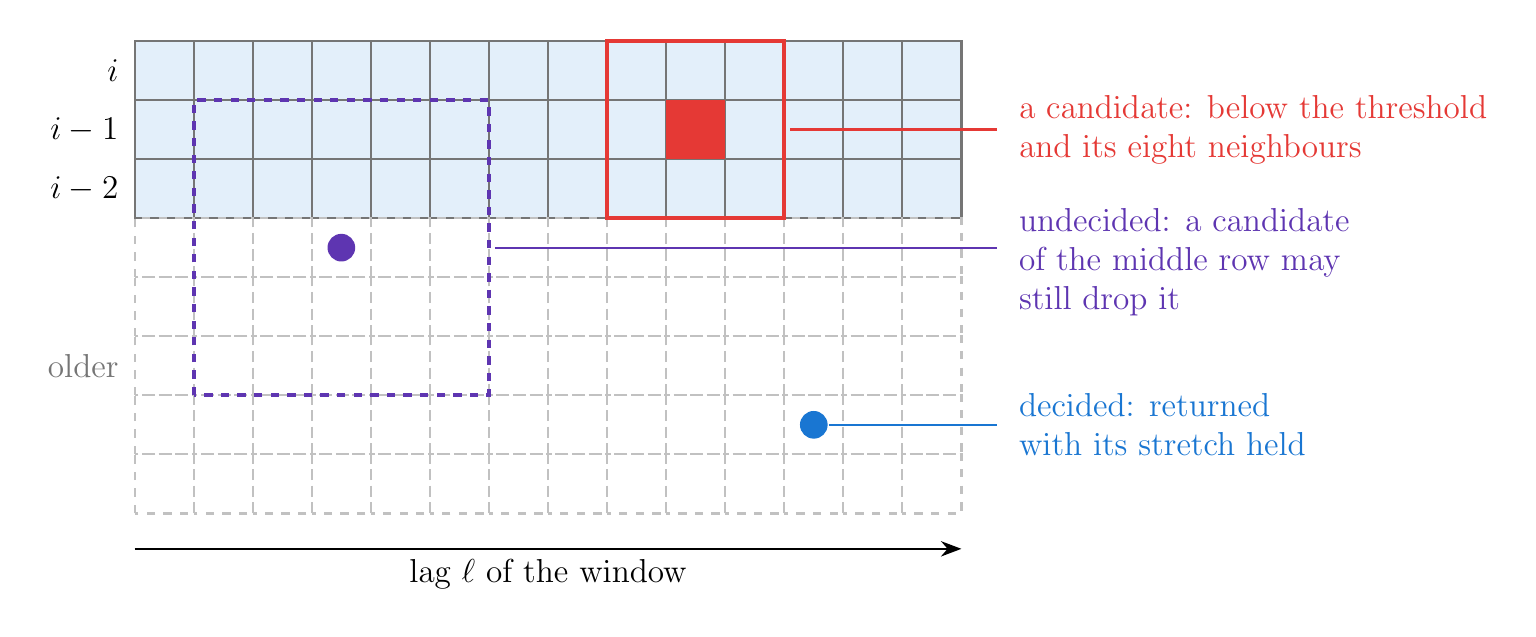
\begin{tikzpicture}[>={Stealth[length=2.6mm]}, every node/.style={font=\large}, x=0.75cm, y=0.75cm,
                    line width=0.8pt]
  % ---- the stored rows and the discarded ones ----
  \foreach \r in {0,...,7} {
    \foreach \c in {0,...,13} {
      \ifnum\r<3
        \draw[cgrey, fill=cblue!12] (\c, -\r) rectangle ++(1, 1);
      \else
        \draw[cgrey!45, dashed] (\c, -\r) rectangle ++(1, 1);
      \fi
    }
  }
  \node[left] at (-0.1, 0.5) {$i$};
  \node[left] at (-0.1, -0.5) {$i - 1$};
  \node[left] at (-0.1, -1.5) {$i - 2$};
  \node[left, cgrey] at (-0.1, -4.5) {older};

  % ---- the test of an entry of the middle row ----
  \draw[cred, line width=1.6pt] (8, -2) rectangle ++(3, 3);
  \fill[cred] (9, -1) rectangle ++(1, 1);

  % ---- an undecided candidate, with its square of side 2W ----
  \draw[cpurple, dashed, line width=1.4pt] (1, -5) rectangle ++(5, 5);
  \fill[cpurple] (3.5, -2.5) circle (5pt);

  % ---- a decided one ----
  \fill[cblue] (11.5, -5.5) circle (5pt);

  % ---- the labels, right of the rows ----
  \draw[cred, line width=0.8pt] (11.1, -0.5) -- (14.6, -0.5);
  \node[cred, right, align=left] at (14.8, -0.5) {a candidate: below the threshold\\ and its eight neighbours};
  \draw[cpurple, line width=0.8pt] (6.1, -2.5) -- (14.6, -2.5);
  \node[cpurple, right, align=left] at (14.8, -2.75) {undecided: a candidate\\ of the middle row may\\ still drop it};
  \draw[cblue, line width=0.8pt] (11.75, -5.5) -- (14.6, -5.5);
  \node[cblue, right, align=left] at (14.8, -5.5) {decided: returned\\ with its stretch held};

  % ---- the axis ----
  \draw[->] (0, -7.6) -- (14, -7.6) node[midway, below] {lag $\ell$ of the window};
\end{tikzpicture}
\end{document}
